\section{Ergebnisse}

\subsection{Vergleich Paramater}
\subsubsection{Taxi}

\subsubsection{Cliff}

\subsubsection{Frozen Lake}

\subsection{Vergleich Algorithmen}

Im folgenden werden die Ergebnisse beschrieben, welche bei dem Vergleichen der Algorithmen Q-Learning und SARSA entstanden sind.
Dabei wurde der Vergleich an den drei Reinforcement Learning Problemen Taxi, Cliff und Frozen Lake durchgeführt. Es wurden jeweils passende Paramater für das entsprechende Problem gewählt.
\subsubsection{Taxi}

In der Abbildung \ref{fig:taxi_train} sind die Ergebnisse für den Vergleich des Q-Learning und SARSA Algorithmus dargestellt. In der linken Abbildung \ref{fig:taxi_rew} sind die Rewards in dem zeitlichen Verlauf über die 3000 Trainingsepisoden abgebildet. Zu erkennen ist hier, dass beide Algorithmen nach ca. 1500 Episoden Richtung Optimum konvergieren. Der Q-Learning Algorithmus trainiert jedoch ein wenig schneller, was durch die anfänglich stärkere Steigung und höheren Peaks zu Beginn verdeutlicht wird.

Zusätzlich ist es auffälig, dass SARSA im späteren Verlauf auch größere Peaks nach unten hate und generell ein wenig schlechter performiert als der Q-Learning Algorithmus. Somit lässt sich insgesamt für die Belohnung feststellen, dass Q-Learning schneller zu einem besseren Ergebnis kommt als SARSA. 

In der zweiten Abbildung \ref{fig:taxi_step} sind die Anzahl der Steps abgebildet, welche der Agent jede Episode durchläuft, bis er entweder bei der maximalen Anzahl angekommen ist oder den Passagier erfolgreich zu seinem Zielort gebracht hat. Der Verlauf der beiden Kurven von Q-Learning und SARSA ist hier sehr ähnlich. Lediglich bei ca. 400 Episoden und 1300 lassen sich leicht höhere Peaks vom SARSA Algorithmus ablesen.
Dies spricht dafür, dass SARSA in diesen Phasen etwas langsamer gelernt hat als der Q-Learning Algorithmus.

Betrachtet man 

\begin{figure}[H]
    \centering
    \begin{subfigure}{.5\textwidth}
      \centering
      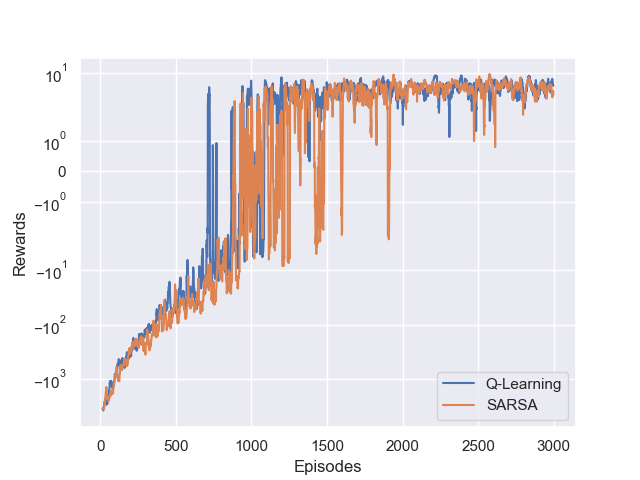
\includegraphics[width=1\linewidth]{taxi_q_vs_s_3000}
      \caption{Rewards}
      \label{fig:taxi_rew}
    \end{subfigure}%
    \begin{subfigure}{.5\textwidth}
      \centering
      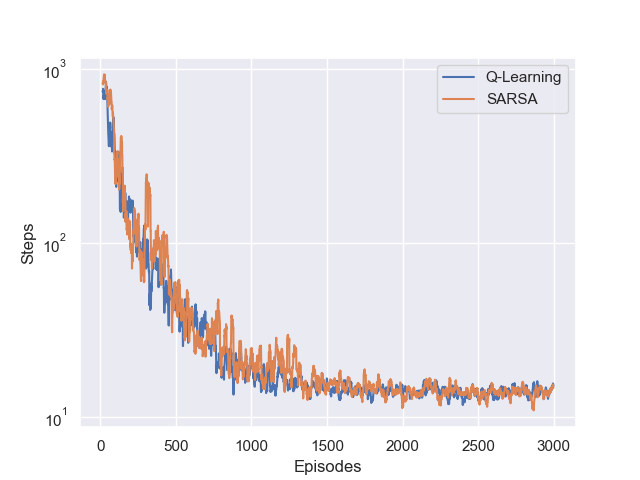
\includegraphics[width=1\linewidth]{taxi_q_vs_s_3000_steps}
      \caption{Steps}
      \label{fig:taxi_step}
    \end{subfigure}
    \caption{Taxi Problem über 3000 Episoden während dem Training}
    \label{fig:taxi_train}
\end{figure}

\subsubsection{Cliff}
\begin{figure}[H]
    \centering
    \begin{subfigure}{.5\textwidth}
      \centering
      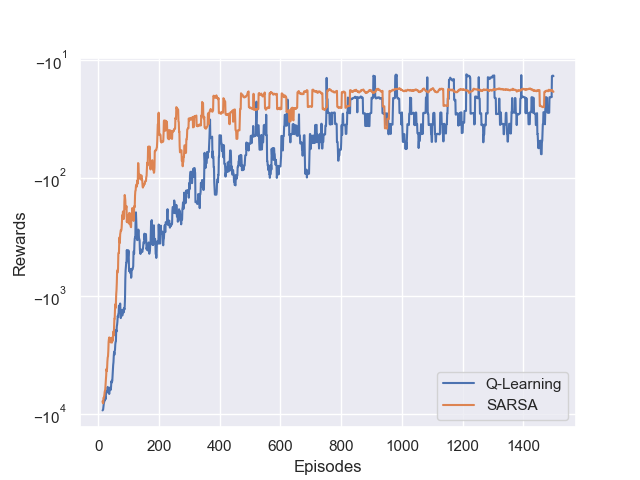
\includegraphics[width=1\linewidth]{cliff_q_vs_s_1500}
      \caption{Rewards}
      \label{fig:cliff_rew}
    \end{subfigure}%
    \begin{subfigure}{.5\textwidth}
      \centering
      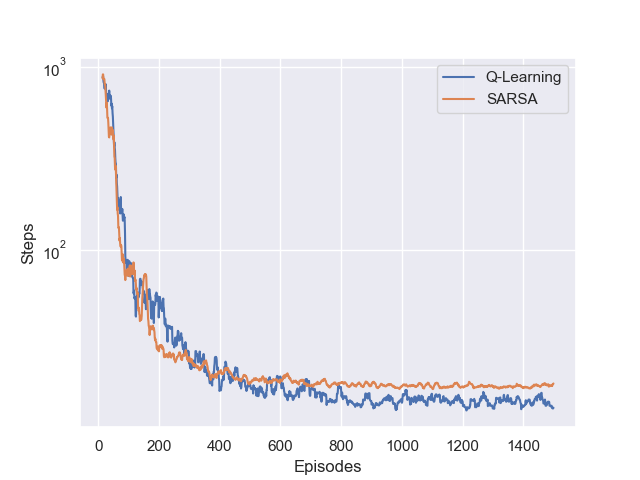
\includegraphics[width=1\linewidth]{cliff_q_vs_s_1500_steps}
      \caption{Steps}
      \label{fig:cliff_step}
    \end{subfigure}
    \caption{Cliff Problem über 1500 Episoden während dem Training}
    \label{fig:cliff_train}
\end{figure}

\begin{figure}[H]
    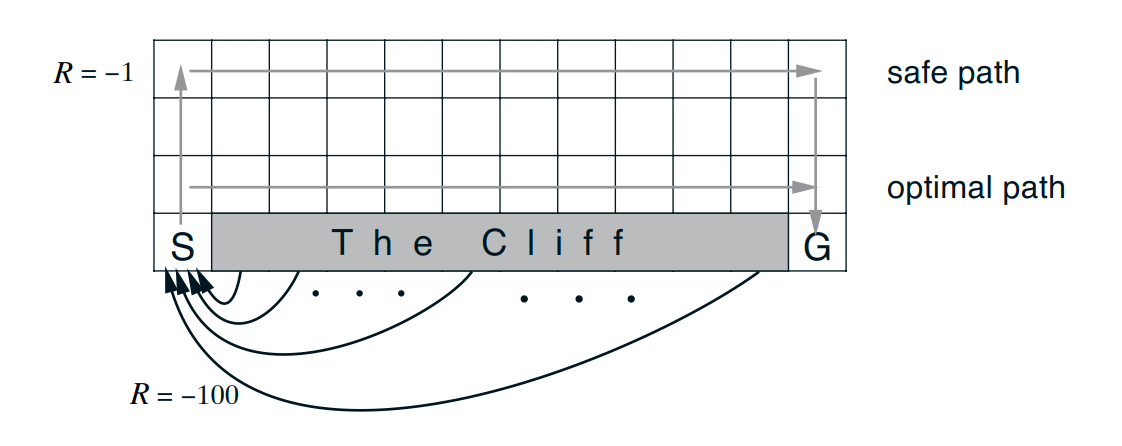
\includegraphics[scale=0.4]{cliff_path}
    \caption{Cliff Q-Learning vs SARSA Pfad}
    \label{fig:cliff_path}
\end{figure}

\subsubsection{Frozen Lake}

\begin{figure}[H]
    \centering
    \begin{subfigure}{.5\textwidth}
      \centering
      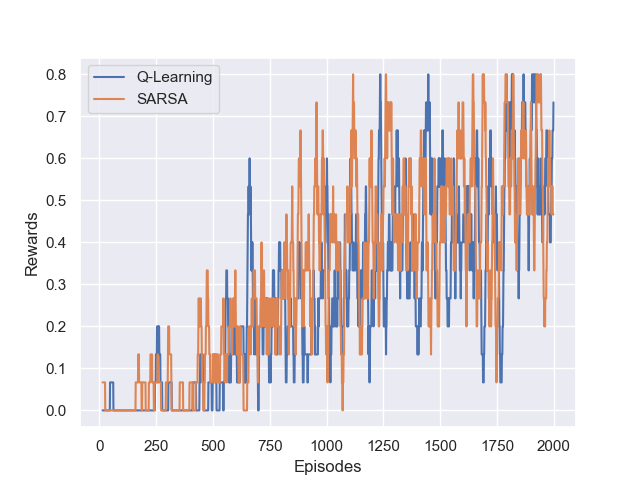
\includegraphics[width=1\linewidth]{frozen_lake_q_vs_s_2000}
      \caption{Rewards}
      \label{fig:frozen_rew}
    \end{subfigure}%
    \begin{subfigure}{.5\textwidth}
      \centering
      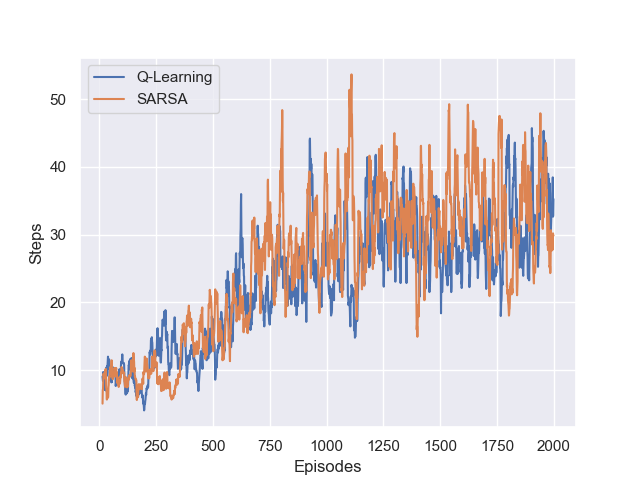
\includegraphics[width=1\linewidth]{frozen_lake_q_vs_s_2000_steps}
      \caption{Steps}
      \label{fig:frozen_step}
    \end{subfigure}
    \caption{Frozen Lake Problem über 2000 Episoden während dem Training}
    \label{fig:frozen_train}
\end{figure}

